\documentclass[11pt,letterpaper]{amsart}
\usepackage{amsmath}
\usepackage{amsfonts}
\usepackage{graphicx}
\usepackage[left=100.00pt, right=100.00pt]{geometry}

\usepackage[dvipsnames]{xcolor}
\usepackage[colorlinks,linkcolor=blue, citecolor=blue,urlcolor=blue]{hyperref}
\usepackage[backend=bibtex]{biblatex}
\usepackage{todonotes}

\newcommand{\R}{\mathbb{R}}
\newcommand{\Q}{\mathbb{Q}}
\newcommand{\N}{\mathbb{N}}
\newcommand{\Z}{\mathbb{Z}}
\DeclareMathOperator*{\qq}{\textit{\textbf{q}}}
\DeclareMathOperator*{\uu}{\textit{\textbf{u}}}

\addbibresource{bib_elastic_coil.bib}


\author{Jason Ngo}
\title{Cosserat model for a circular helix}
\begin{document}
\maketitle
\section{Helix formula}
Given the upright helix $ r(t) = \left(R\cos t, R \sin t, c t\right) $, where $ R $ is the radius of the helix and $ 2\pi c $ is a constant giving the vertical separation of the helix's loops. If $ s $ is the arc-length parameter of the helix, then we have:
\begin{align*}
	s(t) = \int_0^t |r'(t)| d\tau = \int_0^t \sqrt{R^2+c^2} d\tau = \sqrt{R^2+c^2} t.
\end{align*}
Therefore, we can reparametrize the center-line of the helix with respect to the arc-length parameter $ s $ as follows:
\begin{align}\label{eq:r(s)}
	r(s) = \left(R \cos{\frac{s}{\sqrt{R^2 + c^2}}}, R \sin{\frac{s}{\sqrt{R^2 + c^2}}}, \frac{cs}{\sqrt{R^2 + c^2}} \right).
\end{align}

\section{Directors}
Here, we assume inextensibility, which requires $ d_3 $ to be tangent to the center-line; therefore, we have:
\begin{equation}\label{eq:d3}
	d_3(s) = \left(-\frac{R \sin \left(\frac{s}{\sqrt{c^2+R^2}}\right)}{\sqrt{c^2+R^2}},\frac{R \cos \left(\frac{s}{\sqrt{c^2+R^2}}\right)}{\sqrt{c^2+R^2}},\frac{c}{\sqrt{c^2+R^2}}\right).
\end{equation}

Now, since $ \{ d_1, d_2 \} $ spans the plane orthogonal to the center-line, we can first choose $ d_1 $ to be a vector on the plane, then compute $ d_2 = d_3 \times d_1 $:
\begin{align}\label{eq:d12}
	d_1(s) &= \left(-\cos{\frac{s}{\sqrt{R^2 + c^2}}}, -\sin{\frac{s}{\sqrt{R^2 + c^2}}}, 0 \right) \\
	d_2(s) &= \left(\frac{c \sin \left(\frac{s}{\sqrt{c^2+R^2}}\right)}{\sqrt{c^2+R^2}},-\frac{c \cos \left(\frac{s}{\sqrt{c^2+R^2}}\right)}{\sqrt{c^2+R^2}},\frac{R}{\sqrt{c^2+R^2}}\right).
\end{align} 

%\vskip 20pt
%
%\todo{i think the section below is wrong}
%Now that we have a formula for the center-line, let's calculate the orthonormal directors. We choose $ d_3 $ to be the unit vector parallel to the axis of the helix and $ d_2 $ to be tangent to the curve and parallel to the $ xy $-plane (cf. Figure \ref{fig:helixframe}). Then, we have the following directors: 
%\begin{align}\label{eq:ds}
%	d_1(s) &= \left(\cos{\frac{s}{\sqrt{R^2 + c^2}}}, \sin{\frac{s}{\sqrt{R^2 + c^2}}}, 0 \right) \\
%	d_2(s) &= \left(-\sin{\frac{s}{\sqrt{R^2 + c^2}}}, \cos{\frac{s}{\sqrt{R^2 + c^2}}}, 0 \right) \\
%	d_3(s) &= \left(0,0,1\right).
%\end{align}
%
%\begin{figure}[htb!]
%	\centering
%	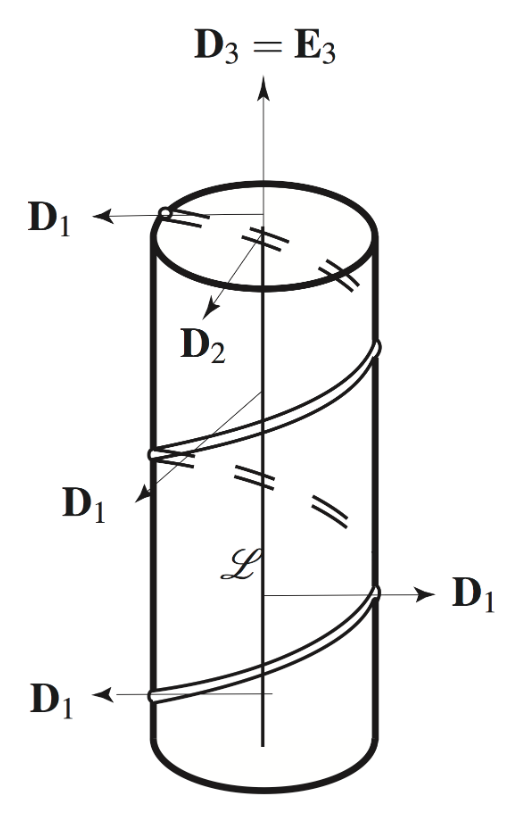
\includegraphics[width=0.25\linewidth]{helix_frame}
%	\caption{Orthonormal directors for helix.}
%	\label{fig:helixframe}
%\end{figure}

\section{Euler parameters $ q_i $}

From the master thesis, we know that the directors and Euler parameters at a point $ s $ are related through the equations
%\begin{equation}
%	d_i(s) = D(\qq(s))d_i(0), 
%\end{equation}
%with $ D(q(s)) $ defined by
%\begin{equation}
%	D(\qq) = \frac{1}{\|\qq\|^2}
%\end{equation}
\begin{align}\label{eq:qs}
d_1 &= \frac{1}{\|\qq\|^2} 
\begin{pmatrix}
q_1^2-q_2^2-q_3^2+q_4^2 \\
2(q_1q_2+q_3q_4) \\
2(q_1q_3-q_2q_4)
\end{pmatrix} \\
d_2 &= \frac{1}{\|\qq\|^2} 
\begin{pmatrix}
2(q_1q_2-q_3q_4) \\
-q_1^2+q_2^2-q_3^2+q_4^2 \\
2(q_1q_4+q_2q_3)
\end{pmatrix} \\
d_3 &= \frac{1}{\|\qq\|^2} 
\begin{pmatrix}
2(q_1q_3+q_2q_4) \\
2(-q_1q_4+q_2q_3) \\
-q_1^2-q_2^2+q_3^2+q_4^2
\end{pmatrix}.
\end{align}

With the additional requirement of $ \|\qq\|^2=1 $, we can compute $ \qq(s) $:
\begin{align*}\label{eq:q}
	q_1 &= -\frac{R \sin \left(\frac{s}{\sqrt{c^2+R^2}}\right)}{2 \sqrt{c^2+R^2} \sqrt{\frac{\left(\sqrt{c^2+R^2}+c\right) \left(\cos \left(\frac{s}{\sqrt{c^2+R^2}}\right)+1\right)}{\sqrt{c^2+R^2}}}}, \\
	q_2 &= \frac{1}{2} \sqrt{\frac{\left(\sqrt{c^2+R^2}-c\right) \left(\cos \left(\frac{s}{\sqrt{c^2+R^2}}\right)+1\right)}{\sqrt{c^2+R^2}}}, \\
	q_3 &= \frac{1}{2} \sqrt{\frac{\left(\sqrt{c^2+R^2}+c\right) \left(\cos \left(\frac{s}{\sqrt{c^2+R^2}}\right)+1\right)}{\sqrt{c^2+R^2}}}, \\
	q_4 &=-\frac{R \sin \left(\frac{s}{\sqrt{c^2+R^2}}\right)}{2 \sqrt{c^2+R^2} \sqrt{\frac{\left(\sqrt{c^2+R^2}-c\right) \left(\cos \left(\frac{s}{\sqrt{c^2+R^2}}\right)+1\right)}{\sqrt{c^2+R^2}}}}.
\end{align*}
%So I first tried \verb|MATLAB| to calculate, but the program gave no explicit solution, so I tried calculating by hand and got the following solution:
%\begin{align*}
%	q_1 &= 0, \\
%	q_2 &= 0, \\
%	q_3 &= \sqrt{\frac{1-\cos{\frac{s}{\sqrt{R^2 + c^2}}}}{2}}, \\
%	q_4 &= - \sqrt{\frac{1+\cos{\frac{s}{\sqrt{R^2 + c^2}}}}{2}}.
%\end{align*}


\section{Strain parameters $ u_i $}
%Now that we have the formulas for the Euler parameter, using the formula:
%\begin{equation}
%	u_i(s) = \frac{2 \frac{d\qq}{ds}^T B_i \qq(s)}{\|\qq(s)\|^2},
%\end{equation}
%we can compute the strain components $ u_i(s) $:
%\begin{align}
%	u_1(s) &= 0 \\
%	u_2(s) &= 0 \\
%	u_3(s) &= \frac{\sin \left(\frac{s}{\sqrt{c^2+R^2}}\right) \sqrt{1-\cos \left(\frac{s}{\sqrt{c^2+R^2}}\right)}}{4 \sqrt{c^2+R^2} \sqrt{\cos \left(\frac{s}{\sqrt{c^2+R^2}}\right)+1}}-\frac{\sin \left(\frac{s}{\sqrt{c^2+R^2}}\right) \sqrt{\cos \left(\frac{s}{\sqrt{c^2+R^2}}\right)+1}}{4 \sqrt{c^2+R^2} \sqrt{1-\cos \left(\frac{s}{\sqrt{c^2+R^2}}\right)}}
%\end{align}
%
%\todo{does this make sense?}

Given the directors, we can compute the strain parameters as follows:
\begin{align*}
	u_1(s) &= -d'3(s) \cdot d_2(s) = 0 \\
	u_2(s) &=  d'3(s) \cdot d_1(s) = \frac{R}{c^2 + R^2} \\
	u_3(s) &=  d'1(s) \cdot d_2(s) = \frac{c}{c^2 + R^2}.
\end{align*}
%
%\vskip 50pt
%
%As a reminder, $ u_1, u_2 $ and $ u_3 $ represent strain with respect to bending,
%
%represent strain with respect to bending, for j = 1,2, and twisting, for j = 3,
%while $ \hat{u}_j $ will represent the intrinsic curvature of the rod for j = 1,2 and the
%intrinsic twist in the rod for j = 3
%
%\vskip 10pt
%
%\todo{consider moving this section}
%curvature:
%\begin{equation}
%\kappa = \frac{R}{R^2 + c^2}.
%\end{equation}
%
%\todo{finish this} 
\end{document}